\providecommand{\sixbysix}{\ensuremath{6\times 6\mathrm{~cm}^{2}}\xspace}
\providecommand{\threebythree}{\ensuremath{3\times 3\mathrm{~cm}^{2}}\xspace}
\providecommand{\twobytwo}{\ensuremath{2\times 2\mathrm{~cm}^{2}}\xspace}
\providecommand{\onebyone}{\ensuremath{1\times 1\mathrm{~cm}^{2}}\xspace}
\providecommand{\relChIso}{\ensuremath{Ch_{iso}/p_T^{muon}}}

\chapter{The HL-LHC upgrade of CMS}
\label{chapter:cms_upgrade}

In this chapter the upgrade of the LHC complex is briefly introduced in Section~\ref{upgrade_lhc}
underlining the physics goal and the expected performance of the machine. The CMS experiment is already planning
a series of upgrades, most of which will be installed during LS3 (Figure~\ref{fig:lhc_plan}).
The overall upgrade project of the CMS detector is outplined in Section~\ref{Sec:upgrade_cms}, with further details on the
foreseen inclusion of time information in the event reconstruction given throughout the rest of the chapter.

\section{High Luminosity LHC}
\label{upgrade_lhc}

The main objective of the High Luminosity LHC (HL-LHC) upgrade [9] of the LHC accelerator complex
is to make precise measurements of the Higgs boson couplings, other rare standard model process (like the vector boson scattering)
and provide a very large dataset ($3000\fbinv$) for new physics searches.
The design include a substantial upgrade of the accelerator complex with the goal of reaching
a peak luminosity of $7.5\times10^{34} cm^{-2}s^{-1}$ (roughly four times as mush as the current value)
The integrated luminosity will about ten times the expected luminosity of the first twelve
years of the LHC.
The timeline of LHC and HL-LHC operation is sketched in Figure~\ref{fig:lhc_plan}, showing the planned
evolution of proton beam intensity through the remaining LHC operating periods (Run 2 and Run 3)
and the HL-LHC operating period following the upgrade of the accelerator complex in LS3.
%The two periods of operation are termed Phase-1 (LHC) and Phase-2 (HL-LHC).

The peak luminosity will be achieved by increasing the beams intensities and by squeezing more the two beams at the
interaction points where ATLAS and CMS are located.
This will lead to a higher number of collisions occurring within the same bunch crossing, the
average number of collisions will increase from 40-60 of LHC to 140-200 at HL-LHC.
The ability of the detectors (ATLAS and CMS) in assigning particles to the correct collision within the same bunch crossing
will worsen with the increased instantaneous luminosity. In order to take advantage of the increased dataset
both experiments are planning to upgrade their detectors to improve the event reconstruction and also improve
the radiation resistance of the detectors components.


\section{HL-LHC upgrade of CMS}
\label{upgrade_cms}
The CMS detector will be upgraded to match the operation environment of HL-LHC in order to fully exploit the
larger dataset delivered by the accelerator complex.
The major points are the complete replacement of the current tracker~\cite{trk_phase2_tdr}, the new system will maintain
the same concept of an all silicon detector with four pixel layers for the precise vertex reconstruction
surrounded by silicon strips devoted to the measurement of the charged particle momentum, but the new detector
will have a finer granularity and an extend pseudorapidity coverage (from the current $|\eta|=2.5$ to $4$).
The finer granularity will mitigate the increased tracks overlap while the extended coverage will provide
a larger acceptance for analysis of interest in the context of HL-LHC.
Contrary to the current system the new tracker will provide information to the Level-1 trigger system,
the information will be exploited to compute isolation quantities and to improve the energy resolution on jets
and $E_T^{miss}$. This improvements are expected to provide a way to control the trigger rate
by improving the event selection already at the Level-1 trigger even with energy thresholds lower than the ones
currently in use, resulting again in an acceptance gain especially for precision measurement of rare standard
model processes.

The Level-1 itself will also be upgraded with a completely new dedicated electronics, the trigger rate
will increase from 100 kHz of LHC to 750 kHz of HL-LHC. The upgrade of the trigger will be matched with
upgrades in most of the sub-detectors electronics to provide information with the higher rate.

The current calorimeter system present in the endcaps will not survive till the end of HL-LHC due to radiation
damage (more than $1.5\times10^{15} n_{eq}/cm^{2}$ in the parts closer to the beam line) affecting the active components of
ECAL (\PbWO crystals) and HCAL (scintillating tiles and photo-detectors).
The two calorimeters will be replaced with a silicon based high granularity sampling calorimeter (HGCAL)
with tungsten absorbers in the
electromagnetic part and lead absorbers in the hadronic one. The longitudinal segmentation will provide
discrimination between overlapping energy deposits.

The muon system acceptance will also be extended up to $|\eta| = 2.8$~\cite{muon_phase2_tdr} with the insertion in
the magnet return yoke of GEM based detectors. This will be beneficial for precision measurement of the Higgs boson
properties through its decay in four muons ($H\to ZZ\to 4 \mu$).

The CMS experiment is also investigating the possible benefits arising from the inclusion of the particles
time of flight information into the event reconstruction. The gain is related to the fact that
collisions overlaps in space within the luminous region but can be separated in time provided a resolution of the
order of $10 ps$ (Figure~\ref{hllhc_beamspot}.
From the knowledge of the production time at the interaction point that of the energy deposits from neutral
particles in the calorimeters these are assigned to the correct collision exploiting the time information.
The improvements is thus bounded to
to measurements: the reconstruction of the time of flight of charged particles to reconstruct the time
of the interaction vertex and the time of energy deposits in the calorimeters. For this reason a new detector
has been propose to measure the time of flight of charged particles while the upgrade of the ECAL barrel and
the design of the new endcap calorimeter are being optimized to provide a time measurement with a precision
of $30$ ps for electrons and photons with an energy greater than $20$ GeV.

Description of the detector technologies and measurements of their time performance are reported in Sections~\ref{sec:tming_rnd},
while examples of performance improvement obtain with simulation studies are described in Section~\ref{sec:timing_perormance}.

\begin{figure}[h!]
  \centering
  \includegraphics[width = 0.45\textwidth]{figures/upgrade/HLLHC_beamspot_T.pdf}
  \includegraphics[width = 0.45\textwidth]{figures/upgrade/HLLHC_beamspot_Z.pdf} \\
  \includegraphics[width = .7\textwidth]{figures/upgrade/HLLHC_beamspot_TZ.pdf}
  \caption{Collision vertex density in the HL-LHC luminous region for one of the possible beam optics configuration.
    The vertex time distribution is shown in the top left plot, the time of the vertex is measured with respect
    the nominal bunch crossing time provided by the LHC clock. The spatial distribution along the beam axis is shown in
    the top right figure while the two dimensional distribution is shown in the bottom plot.
    The distribution are representative of peak instantaneous luminosity of $5\times10^{34} cm^{-2}s^{-1}$ implying
    an average number of collision per bunch crossing of 140. The ultimate HL-LHC performance will reach an average of 200
    concurrent collisions, which will translate in a peak line density of $1.9$mm$^{-1}$ challenging the ability
    of the tracker to correctly assign charged particles to the correct vertex.}
  \label{fig:hllhc_beamspot}
\end{figure}


\section{Detector R\&D for precise time measurement in CMS}
\label{sec:tming_rnd}
Sub nanosecond precision has already been achieved in high energy physics experiments and at LHC.
The current best performances are from the ALICE Time Of Flight system~\cite{alice_tof}, the LHCb TORCH
detector~\cite{lhcb_torch} and the CMS ECAL as described in the following section. The ALICE TOF is
based on the Multi-gap Resistive Plate Chambers capable of a resolution of $80$ ps. The LHCb TORCH
can reach a precision of $50$ ps using Micro Channel Plate (MCP) photo-detectors. Both system are
designed for low energy particle discrimination at low luminosity collider experiments, thus both technology
although already operational at LHC cannot survive the higher irradiation level of CMS during HL-LHC.
The CMS ECAL on the other end is currently limited by clock distribution as explained in Section~\ref{sec:ecal_time_run1}
but is capable of an intrinsic time performance of better than $30$ ps (see~\ref{sec:ecal_time_run1}.

A series of beam test were conducted during 2015 and 2016 to establish the time performances of detector
technologies suitable to be operated in CMS during the HL-LHC phase. These detectors includes silicon
pads for the HGCAL, devices optimized for time measurement of minimum ionizing particles (MIP) and also the study of
the ECAL \PbWO crystals and its HL-LHC readout electronics time performance. Most of the test were performed at
the CERN SPS North area at the H2 and H4 beam lines (more details are given in Section~\ref{sec:tb_2015}) with
a data acquisition system (DAQ), reconstruction and analysis software developed specifically for the needs of
these tests. The reconstruction software is optimized for signals digitized at high frequency (5 GHz),
different algorithms are implemented to extract the amplitude and time information from the peculiar signal shapes of
each of the tested detectors (see Section~\ref{sec:tb_2015}).

During beam test conducted during 2015 the time performance of silicon sensors suitable to be installed
in the future CMS endcap calorimeter has been measured~\cite{hgcal_tb_time}. Several sensors of different
thickness were tested, all of which were $p$-type ($n-on-p$) $5\times 5$ mm$^2$ in effective area.
The results (Figure~\ref{fig:hgcal_time_res}) shows an excellent time resolution for showering electrons with an
energy of 50 GeV. The resolution is found to be better than 20 ps for signals with a $S/\sigma_n > 20$,  where
$S$ is the signal amplitude and $\sigma_n$ is the noise RMS. This figure in the final HGCAL will be achieved for
energy depositions equivalent to 10 MIP. The HGCAL time measurement will also profit from the longitudinal segmentation that will
allow to combine more than one time measurement. Simulation studies shows that a resolution at the level of 20 ps is
achieved for electromagnetic showers with energies above 2 GeV and for hadrons above 20 GeV.

\begin{figure}[h!]
  \centering
  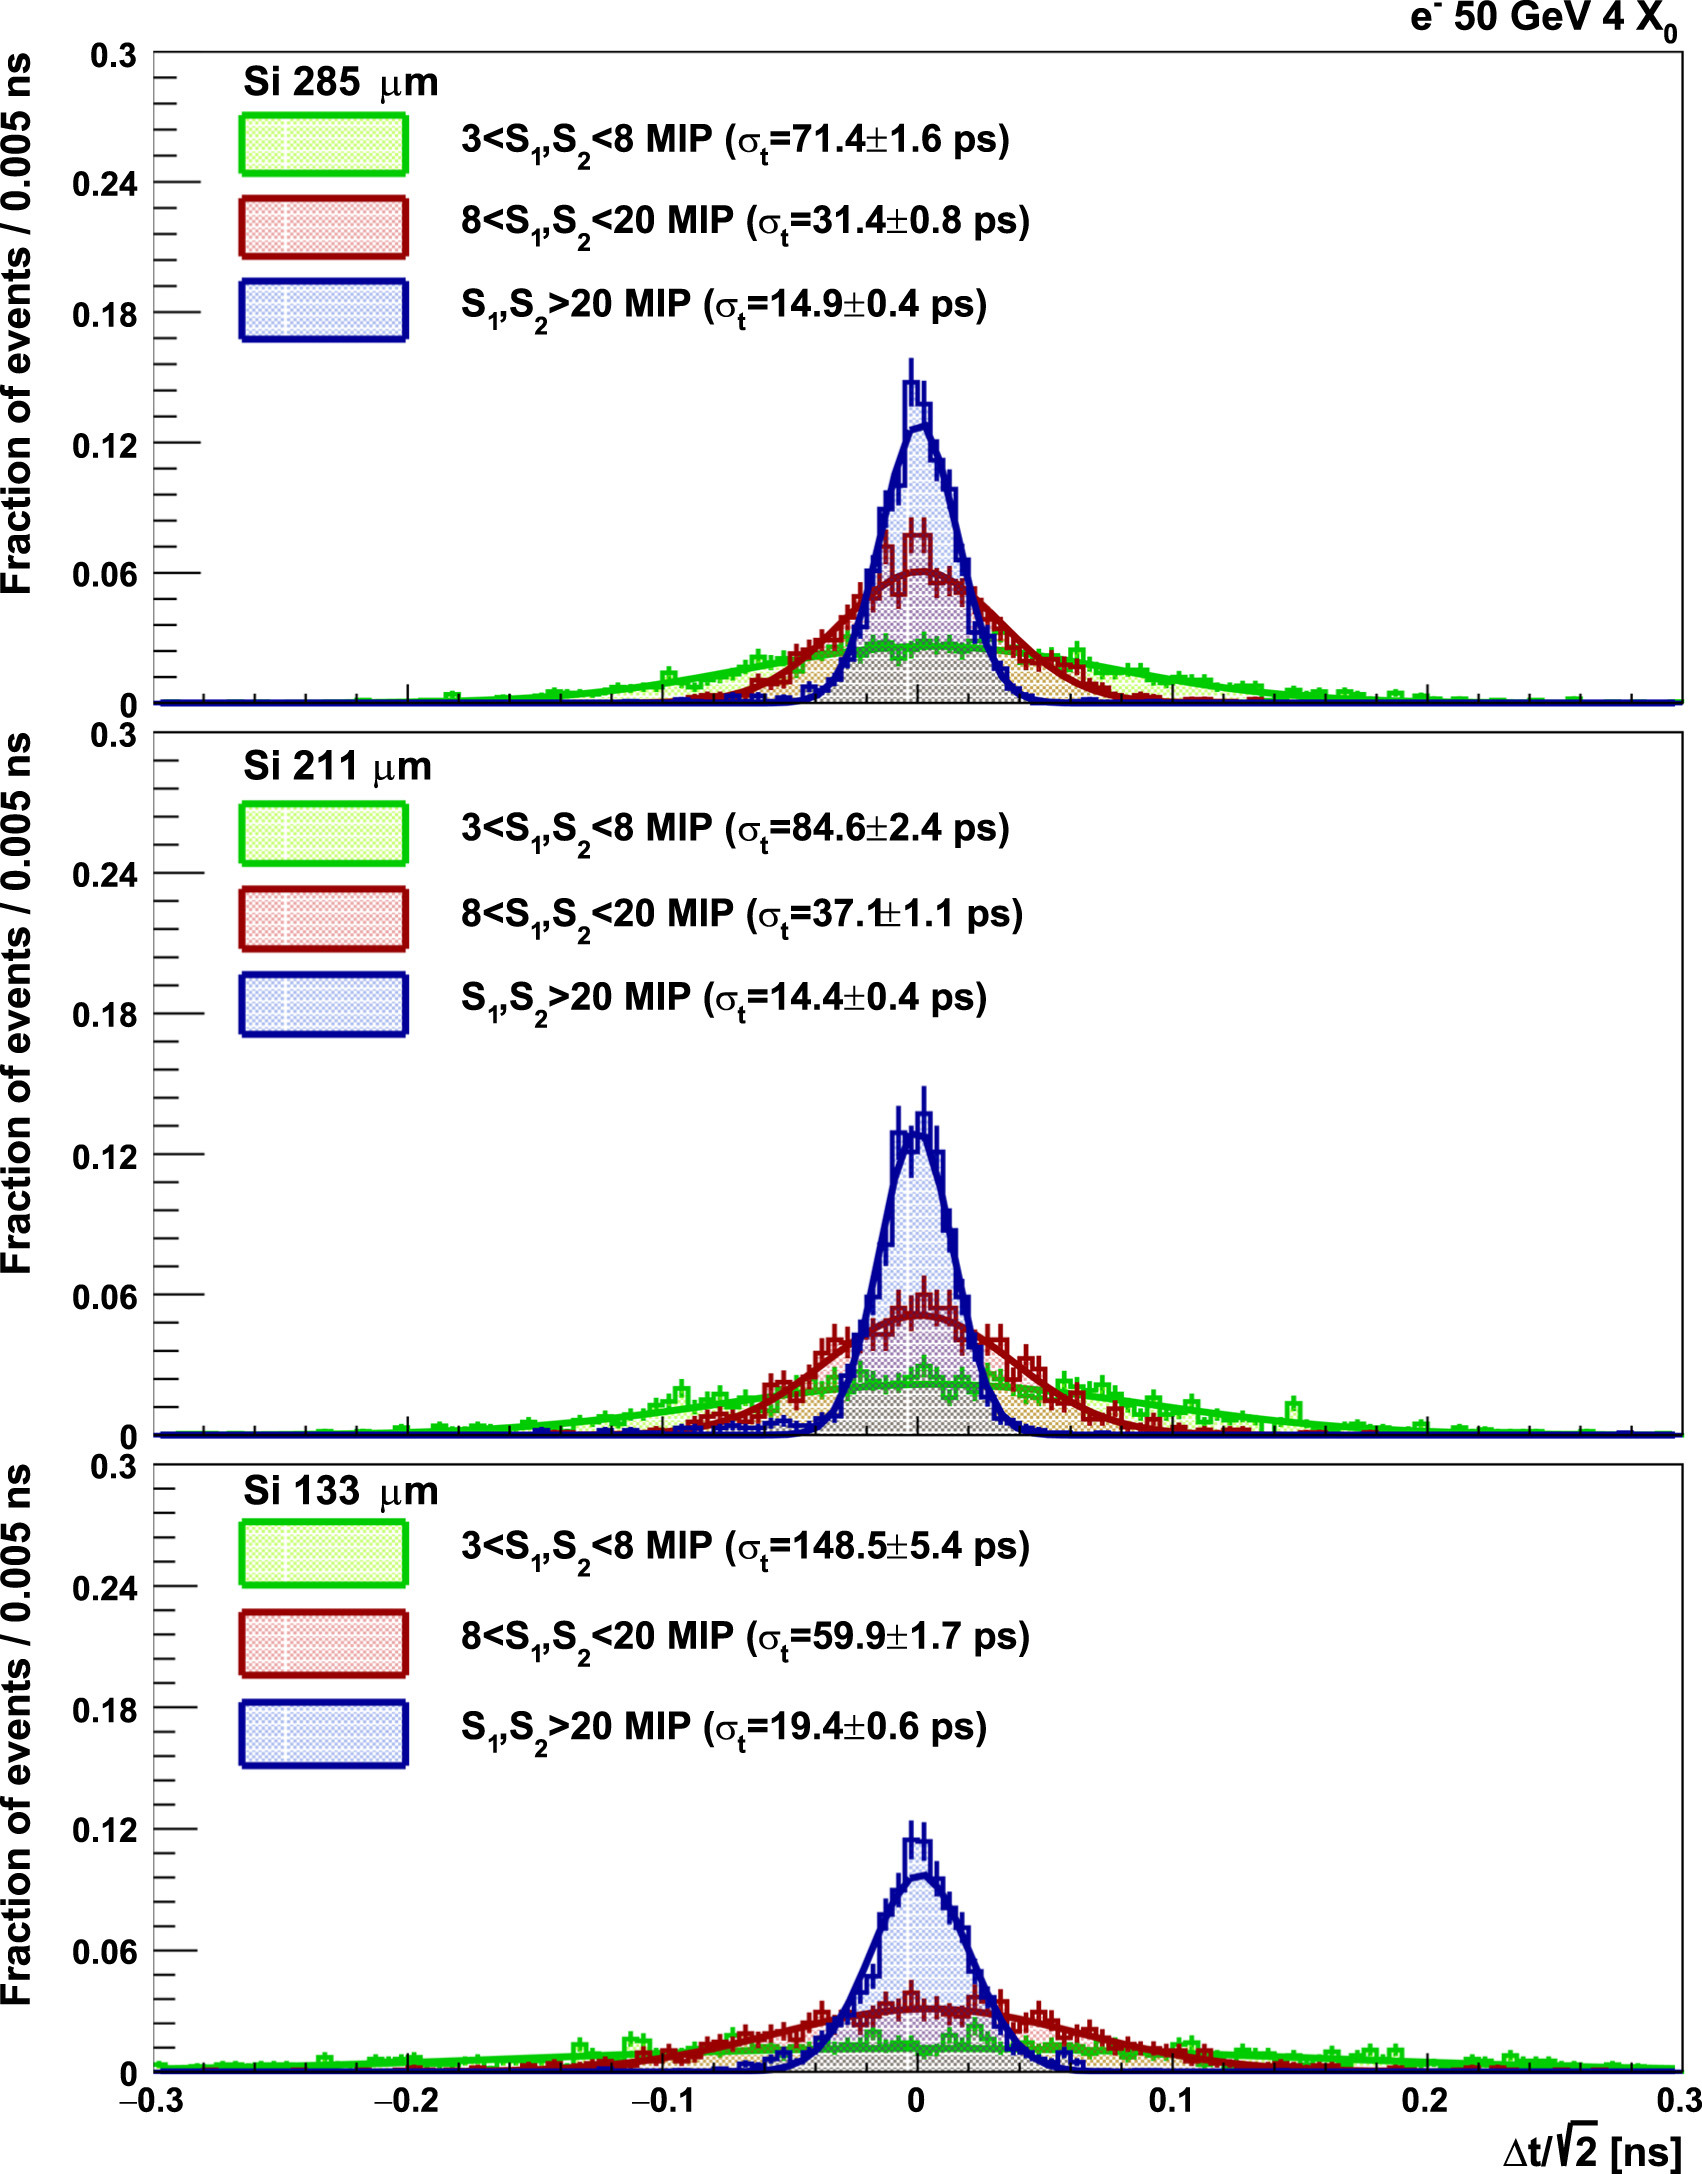
\includegraphics[width = 0.7\textwidth]{figures/upgrade/hgcal_timing.png}
  \caption{The distribution of the time difference between the signals from a pair of silicon sensors ($\Delta t = t_1 - t_2$),
    133-μm (bottom), 211-μm (middle), and 285-μm (top) thick,
    as a function of three different signal ranges as indicated on the upper left corner of each plot.
    The solid lines represent Gaussian fits to the data points.
    The sensors were placed behind a $4X_9$ lead absorber and the electron beam energy was 50 GeV.~\cite{hgcal_time_tb}}
  \label{fig:hgcal_time_res}
\end{figure}
  
The study on the ECAL time performance is reported in details in the next sections. The results show that,
given a clock distribution precision better than 10 ps, a time resolution of 30 ps is achieved at energies
of at least 25 GeV at the beginning of HL-LHC.

These results show the case for the installation of a dedicated detector for the time measurement of charged particles:
none of the existing or foreseen detectors is capable of provide timing information for MIP particles with an
acceptance covering up to $|\eta|\sim 3$ and $p_T > 0.7$ GeV (barrel) or $p > 0.7$ GeV (endcaps).

Given the different irradiation levels and installation schedule constrains, two different
technologies will be adopted for the barrel and endcap timing detectors. In the endcaps (ETL) two planes of
Low-Gain Avalanche Detectors (LGAD) silicon sensors have been proposed since this is the only technology
to survive a dose of $2\times 10^{15} n_{eq}/cm^2$ 
(corresponding to the irradiation level reached after 4000 \fbinv at $|\eta|=3.0$)
while still providing a 50 ps single sensor time resolution~\cite{lgad1, lgad2}. The detector will have
a pseudorapidity acceptance from about $|\eta| = 1.6$ to $|\eta| = 2.9$.

In the barrel region the timing detector (BTL) proposed location is between the silicon tracker and the ECAL, inside the
tracker support structure. This location poses severe constrains on the development and construction of the
timing detector since it will be mounted in the support structure before the tracker sensors. For this reason a
different technology has been chosen for the barrel sensors. LYSO crystals with Ce doping
with a surface of $12\times 12$ and a variable thickness between 3 and 4 mm coupled to Silicon photon multipliers (SiPM)
will form the basic cell of the barrel timing detector. This technology has already been extensively tested
for medical applications (PET), the challenging environment of HL-LHC anyway will require a different optimization
of the geometry. The radiation dose accumulated during HL-LHC will be a order of magnitude lower in the barrel than
in the endcaps making the choice of LYSO crystals and SiPM viable for the BTL but not for the ETL.
Beam test results shows (Figure~\ref{fig:btl_time_res}) that a time resolution of 30 ps is achieved with
a sensor that matches the power consumption and radiation hardness constrains of HL-LHC operation. The test beam
were conducted using the same setup described for the ECAL tests, in particular the same SiPM readout chip was used.
This chip does not provide sufficient radiation tolerance to be operated at HL-LHC. The final readout chip
will be adapted from an existing chip for medical applications.
The time measurement in the barrel sensors is found to depend on the MIP impact position, as shown in Figure~\ref{fig:btl_time_res}
the effect can be corrected to reach a 30 ps time resolution with a spatial precision of 1 mm on the impact point.
Such precision is achieved only for tracks with $p_T > 2$ GeV thus alternative geometries are being investigated.

\begin{figure}[h!]
  \centering
  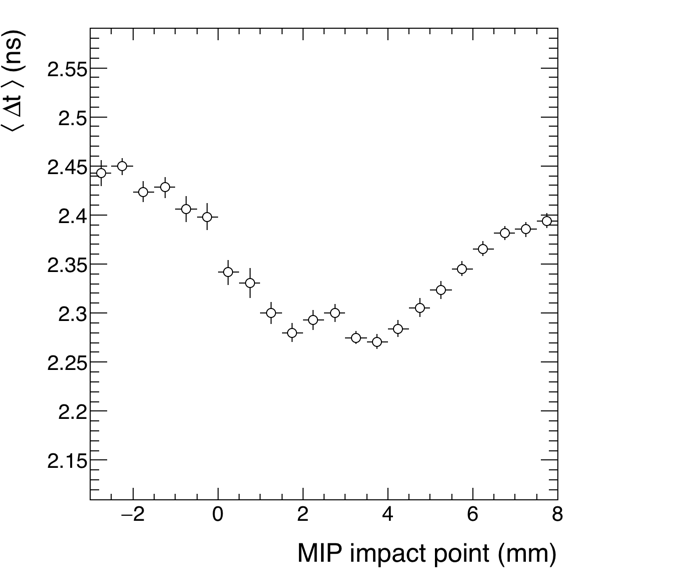
\includegraphics[width = 0.45\textwidth]{figures/upgrade/c_posProfile.png}
  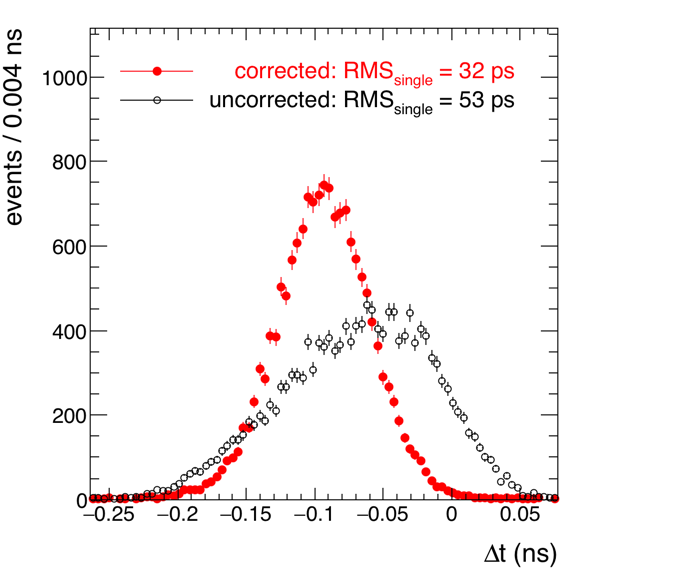
\includegraphics[width = 0.45\textwidth]{figures/upgrade/c_CTR_posCorr.png}
  \caption{Difference between the time measurements in LYSO+SiPM cell and in a reference MCP
    as a function of the MIP impact point on the crystal surface (left).
    Time resolution before and after the application of a position dependent correction (right).}
  \label{fig:btl_time_res}
\end{figure}

\section{The ECAL barrel upgrade}
The primary technical motivation for the ECAL barrel (EB) upgrade is the trigger requirement for
an increase of the trigger latency from about $4\mu$s in the current system [4] to a maximum of $12.5\mu$s,
and a Level-1 trigger rate of up to 750 kHz compared to the current 100 kHz.
The EB electronics Front End (FE) card and all the read-out electronics will be replaced to
meet these requirements. The current configuration provides trigger information to the Level-1
with a granularity of five-by-five crystals, the upgraded system will have a single crystal granularity
enhancing event selection based on isolation information at trigger level which will in turn allow
to set lower thresholds on the transverse energy of the candidate particles.

The foreseen upgraded FE electronics will also provide a shape discrimination between
signal compatible with an electromagnetic shower and those originated from hadronic interaction (``spikes'') in
the photo-detector (APD) which have a narrower shape. The increased Level-1 granularity of a single crystals
will also improve the rejection of such events at trigger level.
The shape discrimination is made possible by a shorter signal shaping performed by the new trans-impedance amplifier
(TIA) and by an ADC with sampling frequency of 160 MHz (four times the current one). The TIA and the increased sampling
frequency is also the key upgrade to provide a time measurement at the $30 ps$ level.

% \subsection{The ECAL timing performance}
% To assess the timing capabilities of the ECAL a series of test beams have been carried out during the R\&D phase.
% The test beam goal is to first measure the intrinsic time resolution achievable with \PbWO crystals and
% APD system and at a second stage verify the performance with the sampling frequency of 160MHz.

\subsection{The current ECAL timing performances}
\label{sec:ecal_time_run1}
The time of an electromagnetic shower in the ECAL is defined as the time at which the signal generated
in the APDs reaches its maximum amplitude. The method to extract this information from the digitized signal
shape is described in \cite{ecal_time_reco}. The time of the maximum $T_{max}$ is estimated with each
available pair of samples (up to nine) as:
\[
T_{max, i} = T_i - T(R_i)
\]
where $i$ is the $i-th$ sample, $T_i$ is acquisition time of the $i-th$ sample and $T(R_i)$ is the time
corresponding to the amplitude ratio $R_i = A_i/A_{i+1}$ and is extracted from a parametrization whose parameters
were measured in a test beam prior the installation of CMS. The error ($\sigma_i$) on each $T_{max, i}$ is estimated as
the product of the derivative of the $T(R)$ function and the uncertainty on $R_i$ which is the sum in quadrature
of three components: noise fluctuations in each sample, uncertainty on the pedestal value subtracted from the measured amplitude
and truncation occurring during the 12 bit digitization of the amplitude.
For signal synchronized with the LHC bunch crossing only four or five of the nine possible amplitude
ratios are used, samples with very small amplitude are discarded. The unique signal time is computed
as the weighted average of the  $T_{max, i}$:
\[
  T_{max} = \frac{\sum_i T_{max, i}/\sigma_i^2}{\sum 1/\sigma_i^2}
\]
and the its error as:
\[
  \frac{1}{\sigma_{T_{max}}^2} = \sum_i\frac{1}{\sigma_i^2}
\]

The time resolution can be parametrized as:
\begin{equation}
  \sigma^2(t) = \left( \frac{N\cdot\sigma_n}{A} \right)^2 + \left( \frac{S}{\sqrt{A}} \right)^2 + C^2  
\end{equation}
\label{eq:general_time_res}

where A is the measured signal amplitude, $\sigma_n$ is the RMS of the noise for each sample and
N, S, C represent the noise, stochastic, and constant term coefficients, respectively.
The stochastic term S is related to fluctuations in the collection times of scintillation photons due to
the finite time their emission.

% It was verified in \cite{ecal_time_reco} to have a negligible impact on
% the time resolution expetially when looking at the time difference for two crystals hit by the same electromagnetic
% shower . 

The time performance of the ECAL has been estimated both during the pre-installation test beam \cite{ecal_time_reco}
and with data collected during the 8 TeV operation of LHC \cite{delRe_time_ecal}.
In the test beam measurement the resolution was extracted from the time difference between the two most energetic crystals
of the same electromagnetic shower, in this configuration the stochastic term that appears in Equation~\ref{eq:general_time_res}
can be neglected since shower fluctuation effects cancels out in the difference, Equation~\ref{eq:general_time_res} thus becomes:
\begin{equation}
  \sigma^2(t_1 - t_2) = \left( \frac{N\cdot\sigma_n}{A_{eff}} \right)^2 + 2 \cdot C^2
\end{equation}
\label{eq:ecal_time_res}
Where $A_{eff} = A_1A_2/\sqrt{A_1^2+A_2^2}$ and $t_{1,2}$, $A_{1,2}$ refers to the times and amplitudes measured by the two crystals. 
The time resolution $\sigma(t_1-t_2)$ was estimated with a Gaussian fit to the time difference.
The results obtained in the analysis report a constant term of $20 \pm 4$ ps which, together with a noise term $N = 35.1\pm 0.2$ ns,
gives and expected time resolution better than 100 ps for energy deposits greater than 20 GeV in the barrel.

The prediction was tested with data collected during 2011 and 2012 from CMS. With collisions events it is possible to
test the performance of the whole system including the clock distribution. \Zee events where used in \cite{delRe_time_ecal}
the results show a good performance when measuring the time difference for channels belonging to the same readout unit while
an increasingly poorer performance for channels in different readout units but same shower and channels belonging to
the two different super-clusters in \Zee events (Figure~\ref{fig:ecal_runI_time}).

\begin{figure}[h!]
  \centering
  \includegraphics[width = 0.45\textwidth]{figures/upgrade/t_res_sameRO.pdf}
  \includegraphics[width = 0.45\textwidth]{figures/upgrade/t_res_diffRO.pdf}\\
  \includegraphics[width = 0.5\textwidth]{figures/upgrade/ecal_resol_Z.pdf}
  \caption{Resolution of time difference between the two most energetic crystals of an ECAL cluster as a function of the
    effective amplitude $A_{eff}$, normalized to the noise in the ECAL Barrel for 2011+2012 data,
    for crystals belonging to the same readout unit (top left), different readout unit (top right) and the two most
    energetic crystals in each of the super-clusters generated by electron from \Zee decays (bottom).
    For electrons from Z boson decays the time of each crystals is corrected for the time of flight from the common
  interaction vertex.}
  \label{fig:ecal_runI_time}
\end{figure}

These results were interpreted to be due to time jitter introduced by the clock distribution system and not corrected by
the calibration performed with low energy deposits. The clock stability has been measured in 2016 using laser monitoring data
and while the time resolution constant term is found to be below $40 ps$ even for crystals belonging to different readout unit,
instabilities of the clock synchronization at the level of $100 ps$ were observed over the course of few days. The
observed effect is in agreement with the constant term measured using \Zee events that are collected over a long period of time.

\subsubsection{Beam test setup}
\label{sec:tb_2015}
During 2015 and 2016 a series of tests with electron beam were performed to evaluate the time performance
of the \PbWO crystal plus APDs photo-detectors system and that of the proposed HL-LHC ECAL electronics.
The tests differ from the one conducted before the CMS installation since the time of the electron measured by the
crystal is compared to an external reference provided by a multi-channel-plate based detector (MCP) instead of to an adjacent
crystal hit by the some shower.

The tests were conducted at the CERN SPS north area with a configurable beam of electrons with energies between 20 and 250 GeV.
The electron beam is a secondary beam created from the primary proton beam, extracted from the SPS, using a converter.
The primary beam hits a metallic target producing a variety of particles that are selected through a system of magnets, collimators
and additional targets. The beam line used for the tests can reach a electron purity of $99\%$ and can also be
configured to provide a equally pure pion beam to study ``spikes'' in the APDs.
The beam in the SPS is composed of several bunches that are extracted in an interval of 4-5 s every 14-48 s depending on the
SPS cycle configuration. The extraction line is configured in a way to destroy the bunch scheme of the SPS beam in order
to provide a uniform and less intense beam to the test area.
The energy of the secondary beams of electrons, positron, muons and charged pions can be selected within the 10 to 400 GeV
range. 

The experimental setup included a $5\times 5$ \PbWO crystal matrix identical to those installed in the ECAL barrel,
with two APDs glued at the back (A schematic view of the setup is shown in Figure~\ref{fig:tb_setup}.
In a first beam test, the APDs signals were amplified with the same $CR-RC$ circuit installed in the current ECAL
supermodules, the shaping time for some of the channels was set to 21.5 ns (half of the current one) to match the
one proposed for the HL-LHC upgrade.
The amplified signal was digitized with a 5 GSample/s commercial digitizer (CAEN V1742 VME board)
instead of the final design DAC with 160 MHz sampling frequency.
In order to estimate the impact of fluctuation in the light production depth on the time resolution,
two of SiPM arrays were glued to the front face of the central crystal.
The CAEN digitizer was used to readout also the signals two of SiPM.
In a second test a prototype of the HL-LHC readout electronic was installed in place of the
CR-RC amplification. The signal from the TIA amplifier was digitized with the same VME board and the
160 MHz sampling ADC simulated at the analysis level by sampling the signal shape acquired at 5 GHz by the CAEN digitizer.
This second setup included also two identical MCP to directly estimate their time resolution.

The crystal matrix and readout electronics was kept at $18^{\circ}$ inside box to avoid
light induced noise in the photo-detectors. The reference MCP detector was placed in front of the box. 
Incoming charged particles produce Cerenkov radiation in a quartz window coupled to a photo-cathode,
the photo-electrons produced by the Cerenkov light hitting
the photo-cathode are amplified by two layers of MCP and collected to the anode. 
The MCP device used in the test was characterized 
in a different tests~\cite{mcp1,mcp2} and its time resolution measured to be $25\pm5$ ps.
The signal from the MCP was also digitized with the same CAEN board.

\begin{figure}[h!]
  \centering
  \includegraphics[width = .7\textwidth]{figures/upgrade/tb_setup.pdf}
  \caption{Schematic of the beam test setup (not to scale), the electron beam comes from the left side.
    The \PbWO crystal is drawn in green and the shape is simplified with
    respect the real trapezoidal one. The plastic scintillators described in the text are not drawn and were placed
    upstream of the hodoscope (to the left of HODO in the picture). As in the standard ECAL crystals the signals from the two APDs
    glued on the rear face are merged before the preamplifier (VFE in the scheme).}
  \label{fig:tb_setup}
\end{figure}
  
The setup was complemented by a set of wire chambers and scintillating fibers hodoscopes to measure the position in the plane
transverse to the beam direction (x-y plane) of particles hitting the experimental setup.
Each hodoscope is composed by a set of 64 fibers and has a spatial resolution of 0.5 mm and was placed
3 meter upstream of the crystals box and the MCP. The beam divergence is negligible and thus the impact point on the crystals
face corresponds to the particle transverse position measured by the hodoscopes (Figure~\ref{fig:crystal_amp_map}).

Incoming particles were also detected by three plastic scintillators placed few meters upstream of the crystals position, the
three scintillation signal are discriminated and a trigger for the acquisition system is build as a coincidence of the three signals.
The three scintillators dimensions are \sixbysix, \threebythree, \onebyone, the smallest one selects event impinging at the
center of the \twobytwo crystal front face.

\begin{figure}[h!]
  \centering
  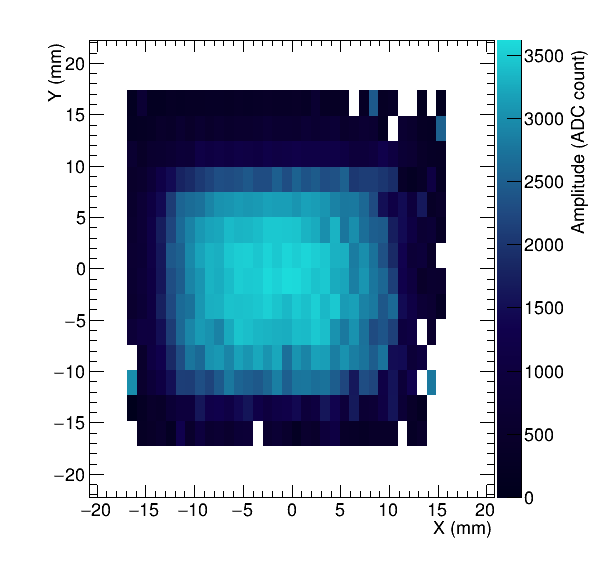
\includegraphics[width = 0.7\textwidth]{figures/upgrade/crystal_amp_map.pdf}
  \caption{Distribution of the signal amplitude of a single crystals as a function of the transverse impact position for
    a 50 GeV electron beam. For alignment purposes the events shown in the picture
    were acquired requiring only the coincidence between the \sixbysix and \threebythree scintillators.
    The crystal front face is a square with 22 mm sides, the area covered by the crystal is clearly visible in the amplitude
    profile as the light area at the center.}
  \label{fig:crystal_amp_map}
\end{figure}

\subsubsection{Amplitude and time reconstruction at the beam test}
The CAEN digitizer has 32 channels and for each event and channel acquires 1024 samples (one every 200 ns). The
digital conversion is performed by a 12-bit DAC, the dynamic range of the DAC is 1 V.
The channels are synchronized at a level better than 5 ps.
The samples were shipped to a commercial PC through the VME bus and an optical interface, the event
synchronization between the digitizer, hodoscopes and wire chamber data was performed by software running on the
acquisition PC.

The MCP signal is very fast, lasting 4 ns, its amplitude is estimated with a second order polynomial fit to the seven samples
around the maximum one while the time extracted with a constant fraction method to avoid amplitude walk effects.

The signal from the SiPM is readout through a NINO chip that provides both the time and amplitude measurements.
The signal time is extracted with a precision under 10 ps as the the time at which the signal pass a threshold that
can be configured. This method is very sensible to the amplitude walk effect and the measured time is therefore
corrected during the analysis.

The amplitude and time of the APD signal are estimated with a template fit to the signal shape where the signal
amplitude and time of the maximum are free to float.
The template shape is build as the average of $1\times 10^5$ signals aligned using the time of the MCP signal
in the same event and scaled by the amplitude estimated with the same approach used for the MCP signal.
A different template shape is constructed in this way
for each crystal. Two template examples are shown in Figure~\ref{fig:apd_templates} for channel with different  
shaping times. The template fit gives the best time performance for APD signals which has a smaller $dV/dt$ compared
to the MCP one.

\begin{figure}[h!]
  \centering
  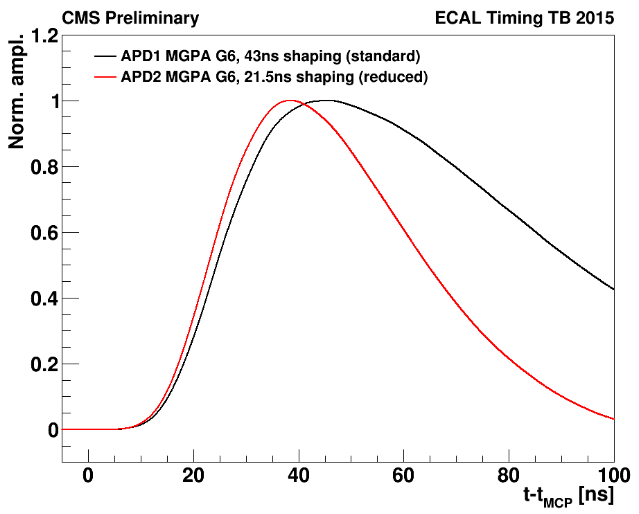
\includegraphics[width = 0.7\textwidth]{figures/upgrade/wf_shaping_times.png}
  \caption{APD signal average shape for 21.5 ns and 43 ns shaping times.}
  \label{fig:apd_templates}
\end{figure}

\subsubsection{Beam test results}
\label{sec:tb_2015_results}
The resolution of the \PbWO crystals plus APDs system is extracted from 
the distribution of the time difference between the time measured by the MCP ($t_{MCP}$) and the crystal ($t_{APD}$)
hit by the electron.
A Gaussian function is fit to the distribution and the standard deviation extracted from the fit is quoted as
the time resolution. The operation is performed at different energies and for two channels with different
amplifier shaping times. Only events in which the electron entered the crystal within 1.5 mm from the center of the
front face where selected. 

Figure~\ref{fig:results_treso} shows the results for the two different shaping times.
The resolution as a function of $A/\sigma_{n}$ is parametrized by the same Formula~\ref{eq:ecal_time_res} used in the
pre-installation test beam adjusting the constant term to take into account the known MCP resolution:
\[
  \sigma^2(t_{APD} - t_{MCP}) = \left( \frac{N\cdot\sigma_n}{A} \right)^2 + C^2 + C_{MCP}^2
\]
where $A$ and $\sigma_n$ are the average amplitude and noise of the APD signal at a given energy, $C_{MCP} = 25 ps$ is
the MCP time resolution and $N$, $C$ are the noise and constant term of the ECAL channel which are free to float in the fit.
As expected, for the same beam energy, the shorter 21.5 ns shaping has a larger amplitude than the 43 ns shaping one,
however in the fit data from both configurations are used.

The measured constant term is $27 \pm 5 ps$ compatible with the $20 \pm 4 ps$ value measured at the
pre-installation test beam comparing the time of two crystals inside the some electromagnetic shower.
The uncertainty on the constant term measured in the 2015 beam test takes into account the 5 ps uncertainty
on the MCP resolution.

\begin{figure}[h!]
  \centering
  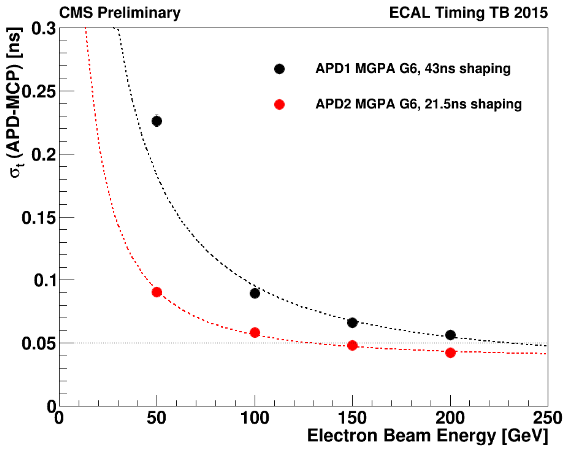
\includegraphics[width = 0.45\textwidth]{figures/upgrade/APD_t_res_vs_energy.png}
  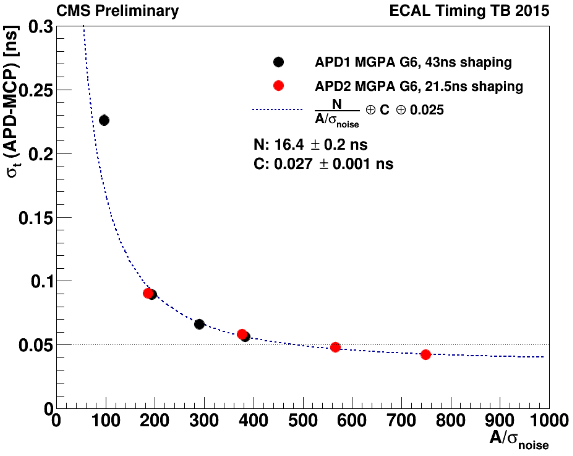
\includegraphics[width = 0.45\textwidth]{figures/upgrade/APD_t_res_vs_AoverN.png}
  \caption{Time resolution on $t_{APD}-t_{MCP}$ as a function of the beam energy (left)
    and the average signal $A/\sigma_n$ (right).
    In the left plot the lines are drawn to guide the eye while in the left plot the curve is the result of the
    fit described in the text.}
  \label{fig:results_treso}
\end{figure}

The test with the HL-LHC electronics prototype again proves a time resolution with a constant term
better than $20$ ps ($17.9\pm 0.1$ ps, Figure~\ref{fig:tia_tres}) with also an improved noise term, as expected
from the TIA.
As explained above the TIA output signal was digitized at 5 GHz and the lower sampling frequency were emulated at the
analysis level. In Figure~\ref{fig:tia_res} the different sampling frequency performance are compared:
the 160 MHz sampling is identical to the one obtained with 5 GHz while at 80 MHz the time resolution
depends on the sampling phase as expected given the typical APD signal frequency spectrum. 

\begin{figure}[h!]
  \centering
  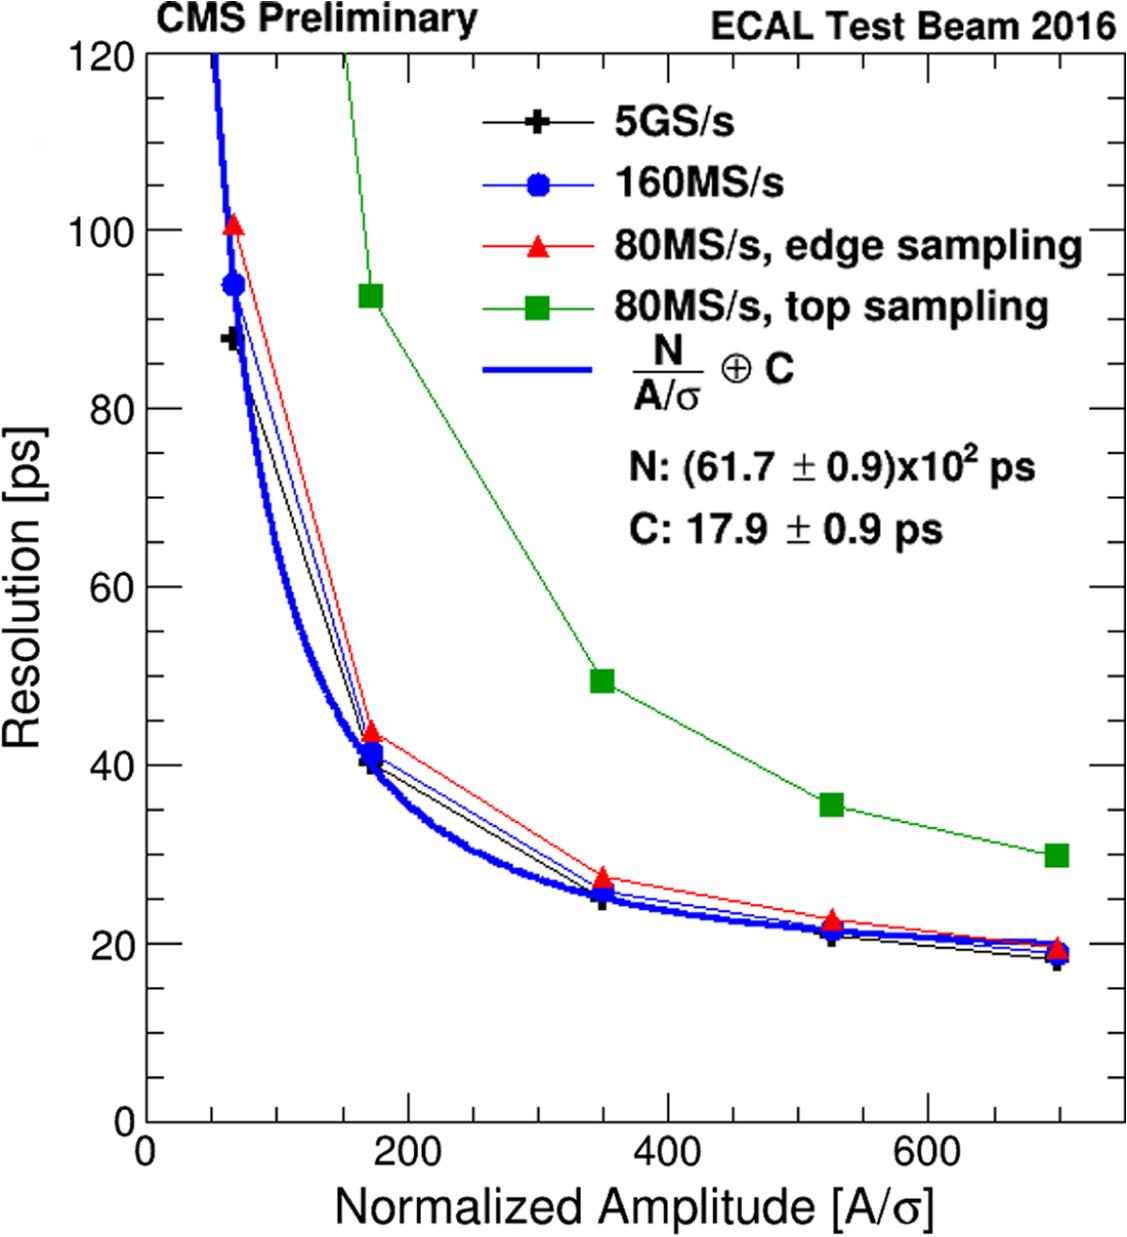
\includegraphics[width = 0.7\textwidth]{figures/upgrade/sampling_freq_res_comp.png}
  \caption{Time resolution performance of HL-LHC ECAL readout electronics for different sampling frequency.
    The baseline 160 MHz sampling frequency does not limit the time performance while the 80 MHz sampling
    performance depends on the phase between the electronics clock and the APD signal.}
  \label{fig:tia_tres}
\end{figure}

The impact of fluctuation in the light production depth on the time performance is estimated comparing the
time performance of the SiPM with that of the APDs. As illustrated in Figure~\ref{fig:light_collection_scheme}, 
the electromagnetic shower propagates faster than the scintillation light in the crystal by a factor equal
to the \PbWO refractive index ($n=2.2$). The different propagation velocity can spoil the time resolution and the
effect is maximized when collecting the scintillation light on the front face since light produced later, deeper in
the crystal also travels a longer minimum path to reach the photo-detector on the front face than the one on the rear face.

\begin{figure}[h!]
  \centering
  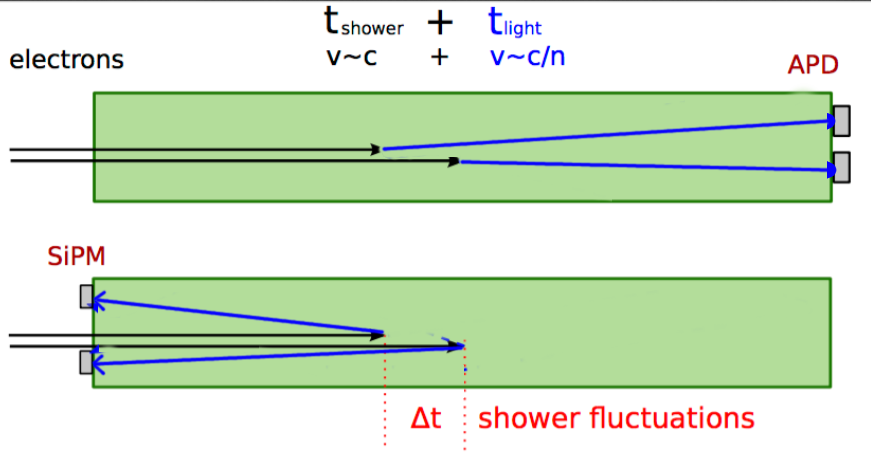
\includegraphics[width = .6\textwidth]{figures/upgrade/shower_fluct_cartoon.png}
  \caption{Illustration of light collection on the front and back face of the \PbWO crystal.}
  \label{fig:light_collection_scheme}
\end{figure}

The intrinsic time resolution of the SiPM arrays is estimated comparing the time measured by the two different arrays using
the same procedure described for APD and MCP comparison. In this comparison shower depth fluctuations cancels since
are common to both SiPM arrays.
The result and the fit are shown in Figure~\ref{fig:sipm_tres},
the fitted time resolution constant term is 25 ps comparable to that of the APDs.
The time resolution is worse when comparing the time measured by one of the SiPM arrays to the one recorded by the MCP,
showing that fluctuation in the light emission depth impact the time resolution adding $\sim 80$ ps in quadrature regardless
of the shower energy. The effect is not seen in the APD performance, proving that the light collection from the rear crystal
face gives the best timing performance.

\begin{figure}[h!]
  \centering
  \includegraphics[width = .7\textwidth]{figures/upgrade/sipm_50um_intrinsic.pdf}
  \caption{Front face light collection time performance. The times measured with the two SiPM arrays
    is compared to the MCP time (grey curves) and one to the other (red curve). SiPM time performance is comparable
    to the APDs one (red) but is affected by light emission fluctuations when comparing to an external
    reference (i.e. MCP).}
  \label{fig:sipm_tres}
\end{figure}

\section{Impact of timing on physics analysis at HL-LHC}
\label{sec:timing_perormance}
The inclusion of per-particle time measurement provide benefits for various physics analysis that are part of
the HL-LHC physics scope.

The time information, as explained at the beginning of the chapter, will improve the vertex reconstruction as
well as the particle to vertex association, in particular the MIP time detector (MTD) will reduce the
number of tracks wrongly assigned to the primary vertex (PV) of each bunch-crossing.
In the context of the CMS technical proposal for HL-LHC the impact of timing on the objects reconstruction and
identification has been studied together with the resulting gain for analysis that are part of the physics scope
of HL-LHC.
Improvements are found in many areas:
\begin{itemize}
\item Pile-up jet suppression: the number of pile-up jets is reduced by $20\%$ in the barrel and $40\%$ in the endcaps
  while retaining full efficiency on signal jets like those produced in VBS events.
\item Improved jet and $E_T^{miss}$ resolution: the rate of events with $E_T^{miss}>130$ GeV is reduced by
  $40\%$ providing less background for SUSY and Dark matter searches.
\item Thanks to a better primary and secondary vertex reconstruction standard b-tagging algorithms reach
  a performance comparable to that of zero pile-up. The b-tagging improved performance translates into
  a direct gain for the measurement of the Higgs boson self coupling since the most sensitive channels
  are $HH\to b\bar{b}b\bar{b}$ and $HH \to b\bar{b}\gamma\gamma$. 
\item Lepton identification through a better resolution on the charged isolation (Section~\ref{sec:muon_iso}.
\item Reconstruction of the diphoton interaction vertex in $H\to\gamma\gamma$ events thanks to both the photon time
  provided by the ECAL and the vertex time from charged particles detected in the MTD. Search for long lived particles
  decaying in a photon and undetected particle will also profit from the precise identification of the primary and
  secondary vertex position. 
\end{itemize}

In the following sections two of the reconstruction improvements outlined above are described in details:
the muon charged isolation and diphoton vertexing. The time-aware event reconstruction and the implementation
of the simulation used are first introduced in the next section.

\subsection{MTD simulation and time-aware event reconstruction}
The simulation used to assess the performance gain brought to the CMS HL-LHC physics program
includes a modelling of the future CMS detector with the tracker acceptance extend to $|\eta|=4$ and
a muon system coverage up to $|\eta|=2.8$. 
Although the MTD detector is simulated, the time of the charged particles
is computed by applying a smearing of 30 ps to the simulation time recorded in the last tracker layer and by
correcting for the time of flight known from the simulation. A time is associated to each track within the acceptance of the BTL
and ETL, while for all other tracks the time is set to zero and an uncertainty of 150 ps is assigned to it (equal to time
spread of the beamspot).
The vertex reconstruction in the $tz$-plane, i.e. in time and position along the
beam line, is done using a time-aware extension of the deterministic
annealing technique adopted in vertex reconstruction by the CMS experiment~\cite{Chatrchyan:2014fea}.

The method used to assign tracks to a primary vertex (PV) based on the distance between the two. This is a common
method within CMS, a typical selection 
requires $|\Delta z(track, PV)| < 1$ mm, which means that for collision closer than 1 mm the reconstructed tracks are
considered as if they were originating from the same interaction. The time selection is introduced in a similar
fashion by requiring $|\Delta t(track, PV)| < N\times\sigma_t$, where $\sigma_t = sqrt{\sigma_t^{track 2}+\sigma_t^{vertex 2}}$
and $N=3$ is chosen for the current study.

One of the benefits of the time-aware event reconstruction is to separate in time events not resolved by
the tracker. Since the probability of vertex merging strongly depends on the density along the beam $z$-axis the
results are presented as a function of the vertex line density.
The vertex line density distributions for the current LHC beamspot and
two possible HL-LHC scenarios are shown in Figure~\ref{fig:vtx_density}, the ultimate
performance of the HL-LHC is expected to give a maximum line density of $1.9$mm$^{-1}$. This scenario is the one simulated
for the studies presented in the following sections, the beamspot distribution
has a Gaussian shape both in $z$ and $t$ directions, with standard deviations of $4.2$ cm and $150$ ps.

\begin{figure}
  \centering
  \includegraphics[width = 0.45\textwidth]{figures/upgrade/VertexSpot.pdf}
  \includegraphics[width = 0.45\textwidth]{figures/upgrade/VertexDensityPDF.pdf}
  \caption{Spread of the vertices along the beam direction at LHC and HL-LHC with 140 and 200 pileup events. 
    The solid (dashed) line refers to the start (end) of the LHC fill (left).
    Probability density function of the vertex density along the beam axis:
    the modes and the means of the three distributions are 0.3, 1.3, and 1.9~mm$^{-1}$ and 0.2, 0.9, and 1.4~mm$^{-1}$ (right).} 
  \label{fig:vtx_density}
\end{figure}

\subsection{Muon isolation with precision timing}
As explained at the beginning of the chapter one of the goals of the HL-LHC is the precise measurement
of the Higgs boson properties. The four muons final state is the purest decay mode from the experimental point of
view as already demonstrated by the analysis that contributed to the first observation of the Higgs boson.
Furthermore the direct decay of the Higgs boson in two muons is the only decay to second generation
leptons that can be observed at HL-LHC.

The vertex merging occurring with $\Delta z$-based association criterion described in the previous section
directly affects the discrimination power of isolation variables since tracks from an unrelated vertex are
not excluded from the isolation cone of a particle coming from the real hard interaction.
This study focuses only on the charged component of the isolation since charged particles comprise
the largest fraction of hadronic activity in $p-p$ collisions and therefore are the most important contribution
to isolation sums in the context of identifying isolated leptons.

%Simulation studies have been performed to assess the gain in muon identification and background rejection.
Signal muons are selected within a sample of prompt muons originated by a Z boson decay by geometrically matching the reconstructed
muon to a true generator-level muon
Non-prompt muons from semileptonic decays of heavy flavour hadrons in $t\bar{t}$ events are
considered representative of non-isolated, background muons. Muons coming from the decay of the W boson produced
by the top quark decay are rejected based on generator-level information and only muons matching a generator-level
hadronic jet are retained.

The algorithm for the choice of the PV currently in use in CMS is inefficient at 200 pile-up, for this reason
the PV is chosen as reconstructed vertex closer to the simulated position of the hard interaction, this procedure
is done independently for the collection of vertices reconstructed with and without the time information.
This choice provide a fair comparison by decoupling the track-vertex association from the correct choice of the PV.

Muons are selected with a set of criteria based on the current CMS muon reconstruction and identification, with
selection optimized for the HL-LHC conditions. Both prompt and non-prompt muons are required to have $|\eta|<2.8$
(muon system acceptance), $p_T > 20$ GeV and a point-of-closest-approach to the primary vertex that is within 1 mm in the
$z$-direction. In the case of the time-aware reconstruction an additional $|\Delta t(muon, vertex)| < 3\times\sigma_t|$
is imposed.

The charged isolation ($Ch_{iso}$) is computed as the sum of the $p_T$ of all tracks within a cone of radius $R=0.3$ centered
around the muon direction excluding the muon track itself. Only tracks with $p_T > 5$ GeV are considered in the sum.
The isolation selection requirement is set on the relative charged isolation value $Ch_{iso}/p_T^{muon}$.

The $\Delta z$ selection value is optimized by comparing the ROC curves for different selection values.
The ROC (receiver operating characteristic) curve is obtained by plotting the efficiency for
non-prompt muons ($\epsilon_{non-prompt}$) versus prompt muons ($\epsilon_{prompt}$) for a spectrum of possible
\relChIso thresholds.
The 1 mm and 2 mm values are found to provide the best performances, as shown in Figure~\ref{fig:muon_dz_comp}, both
for barrel and endcap muons. The 1 mm selection is chosen as baseline for the study since it also provide the
best performances for jets and $E_T^{miss}$ studies.

%% FIXME

The comparison between the timing and no-timing scenario is shown in Figures~\ref{fig:roc_iso_ratio} and highlight
a clear benefit from the use of timing for working points with $\epsilon_{prompt}> 80\%$.
The performance gain can be expressed either in terms of reduced non-prompt rate a constant prompt efficiency
(bottom panels of Figures~\ref{fig:roc_iso_ratio}) or equivalently as prompt efficiency gain at constant non-prompt
efficiency (right panels of Figures~\ref{fig:roc_iso_ratio}).

\begin{figure}[h!]
  \centering
  \includegraphics[width = 1.\textwidth]{figures/upgrade/roc_iso_and_ratios_BTL.pdf}
  \includegraphics[width = 1.\textwidth]{figures/upgrade/roc_iso_and_ratios_ETL.pdf}
  \caption{ROC curves calculated for a cut-off scan in relative charged isolation for muon candidates
    in the BTL (left) and ETL (right) acceptance.}
  \label{fig:roc_iso_ratio}
\end{figure}

The results as a function of the vertex line density are reported in Figure~\ref{fig:muon_iso_vs_density} and show,
as expected, a higher impact of the MTD for the high density bins. The use of time in the \relChIso computation
gives a $10\%$ increase in the $\epsilon_{prompt}$ with a marginal deterioration of the non-prompt rejection.

\begin{figure}
  \centering
  \includegraphics[width = 0.7\textwidth]{figures/upgrade/comparison_fixed_wp0p05.pdf}
  \caption{The efficiency for prompt and non-prompt muons as a function of the event density
    for a representative operating point selection value common to the MTD and no-MTD scenarios.}
  \label{fig:muon_iso_vs_density}
\end{figure}

Different MTD time resolution performances are compared in Figure~\ref{fig:muon_iso_res_comp}: the gain on $\epsilon_{prompt}$
is retained even for a degraded detector performance of 50-70 ps, comparable to that expected at the end of the HL-LHC era.

\begin{figure}[h!]
  \centering
  \includegraphics[width = 0.7\textwidth]{figures/upgrade/comp_t_resolution_wp0p05.pdf}
  \caption{Muon efficiency for relative charged isolation cut-off of 0.05 for different time resolution assumptions, as
    a function of line density.}
  \label{fig:muon_iso_res_comp}
\end{figure}

The improvement on the charged isolation efficiency are projected onto the $H \to 4\mu$ analysis in terms of
an increased signal acceptance and thus increased of equivalent integrated luminosity.
Both the BTL and ETL contribute significantly to the signal gain shown in Figure~\ref{fig:H_4mu_gain}. The
projection are for a charged isolation working point that provides $\epsilon_{prompt}= 90\%$ in the no-MTD case.
The gain introduced by the use of timing is equivalent to a $20\%$ increase in the signal over square-root of the background
ratio.

\begin{figure}
  \centering
  \includegraphics[width = 1.\textwidth]{figures/upgrade/HZZRapidity_TimingStudy_200PU.pdf}
  \caption{Projections for yield enhancement in $H\to ZZ\to 4\mu$ as a function of the Higgs boson rapidity.
    The distributions are normalized to the no-timing case.}
  \label{fig:H_4mu_gain}
\end{figure}

\subsection{Diphoton vertex identification}
The clean diphoton signature is a prime tool to study the Higgs boson properties
The sensitivity of the measurement depends on the invariant mass resolution of the diphoton pair
and on the quality of the photon identification.
The mass resolution, as explained in Chapter~\ref{chapter:diphotons} in the equivalent context of the search for resonances,
is subordinated to the precision on two measurement: the energy resolution of the ECAL and the precision on the
angle between the two photons related to the identification of the diphoton vertex.
If the longitudinal position of the diphoton vertex is known to better than about 10 mm, the opening angle
resolution contributes negligibly to the diphoton mass resolution~\cite{Khachatryan:2014ira}.
For the reasons detailed in the previous sections this channel will
benefit from the improved acceptance for isolated objects and improved vertex identification
capability provided by track and photon timing information.







\section{Summary}
\label{sec:upgrade_summary}

The HL-LHC era will provide an unprecedented amount of data to the ATLAS and CMS experiments through a record
instantaneous luminosity four times higher than the current LHC maximum. CMS is preparing an upgrade of its
detector to match the radiation hardness requirements of HL-LHC and to fully exploit the larger dataset to
perform precision measurement of rare standard model (SM) processes and extend the searches for new phenomena described by
models beyond the SM.

The inclusion of the time information in the event reconstruction has been proved, through simulation studies,
to provide a unique way to mitigate the deterioration of performance due to pile-up and also open the possibility
to measure observable otherwise inaccessible (mass of long lived SUSY particles). The same simulation
studies underline the importance of an hermetic timing measurement charged particles.

During the past two years a series of beam test have proven the timing capabilities of the existing
ECAL barrel sensors and also those proposed for the implementation of the MTD (LYSO crystal with SiPM photo-detectors for
the barrel and silicon sensors for the endcaps). All the technologies are capable of a resolution better than
30 ps when combined into the CMS reconstruction they provide time measurement for charged particles, high energy photons
and neutral hadrons (endcaps only).

Both the tests described above and examples of performance gain have been discussed in this chapter.











  